\chapter{Interfície d'usuari}
\label{chap:interficie_usuari}

La interfície d'usuari és la part que està més exposada al públic de tot el projecte, ja que és on els jugadors de la botifarra viuran les seves experiències i interactuaran amb altres jugadors. Per tal de tenir clar des d'un principi com es volia estructurar es va dissenyar una maqueta de la mateixa abans de començar a treballar, aquestes maquetes s'han desenvolupat utiltizat Pencil Sketching\footnote{Veure secció \ref{sec:pencil sketcing}.}

\section{Maquetes prèvies}

\begin{figure}[htbp]
\centering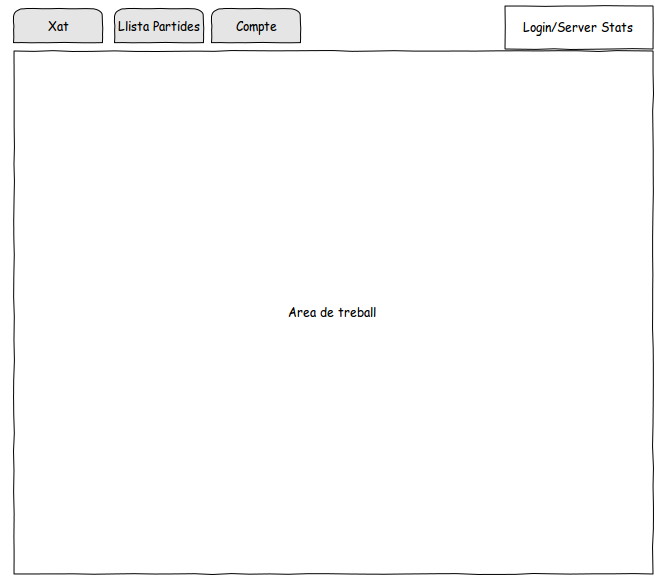
\includegraphics{img/Inici.png}
\caption{Maqueta de la pantalla inicial}
\label{fig:mookup-inici}
\end{figure} 

A la figura \ref{fig:mookup-inici} es pot veure com serà la pantalla inicial. Aquesta s'estructurarà per pestanyes per a que els usuaris puguin accedir a les diferents opcions de la partida. A l'àrea de treball es mostrarà el contingut de les diferents pestanyes. 

\begin{figure}[htbp]
\centering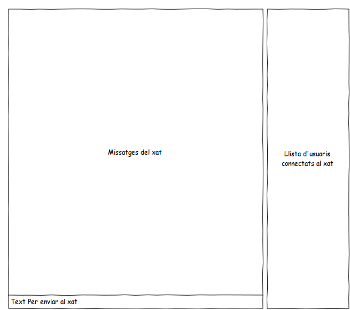
\includegraphics{img/Xat.png}
\caption{Maqueta de la pantalla de Xat}
\label{fig:mookup-xat}
\end{figure} 

A la figura \ref{fig:mookup-xat} es pot veure el contingut que es mostrarà a l'àrea de treball quan la pestanya de xat estigui activa. 

\begin{figure}[htbp]
\centering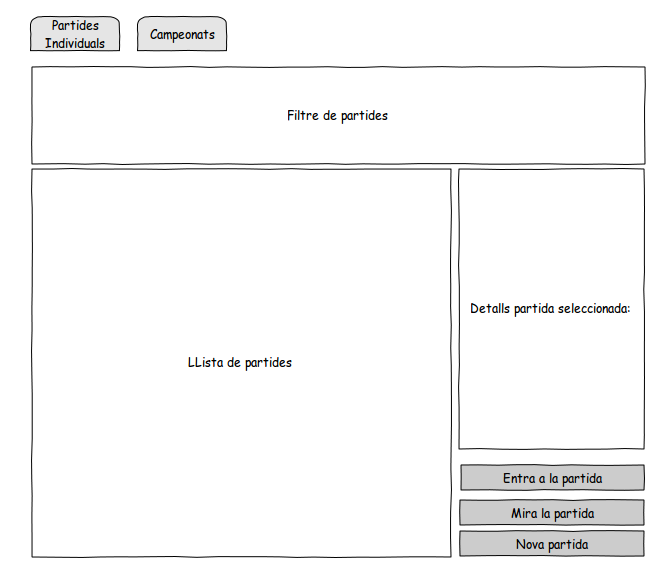
\includegraphics{img/Llista_Partides.png}
\caption{Maqueta del llistat de partides disponibles}
\label{fig:mookup-partides}
\end{figure} 

A la figura \ref{fig:mookup-partides} es pot veure el contingut que es mostrarà a l'àrea de treball quan la pestanya de Llista de partides estigui activa. 

\begin{figure}[htbp]
\centering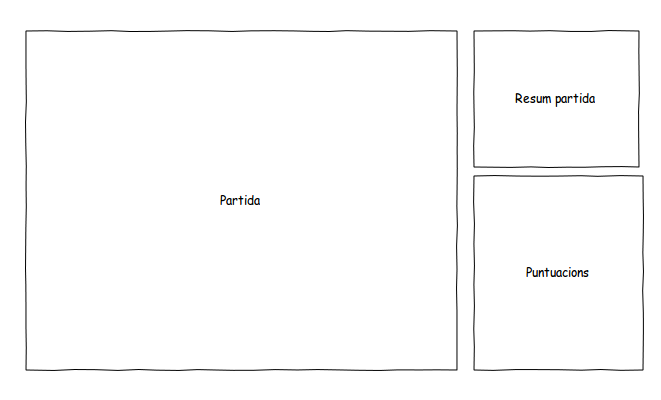
\includegraphics{img/Global_Partida.png}
\caption{Maqueta de la pantalla global de la partida}
\label{fig:mookup-partida}
\end{figure} 

A la figura \ref{fig:mookup-partida} es pot veure el contingut que es mostrarà a l'àrea de treball quan hi hagi una partida en curs. A l'àrea partida serà on els jugadors podran visualitzar el transcurs de la partida i interactuar amb el servidor. Es pot veure en més detall com s'estructura aquesta part en la figura \ref{fig:mookup-detall}.
\begin{figure}[htbp]
\centering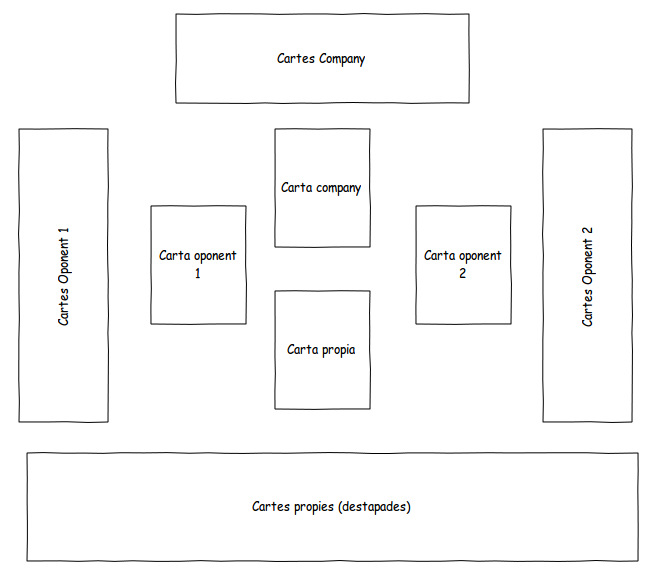
\includegraphics{img/Detall_partida.png}
\caption{Maqueta de la pantalla de detall de la partida}
\label{fig:mookup-detall}
\end{figure} 

\section{Resultat final}

A la figura \ref{fig:real-xat} es pot observar la pantalla que ens mostra l'aplicació després d'identificar-nos. Així al a part esquerra podem veure els missatges del xat i a la part dreta la llista d'usuaris que hi ha connectats al servidor. 

\begin{figure}[htbp]
\centering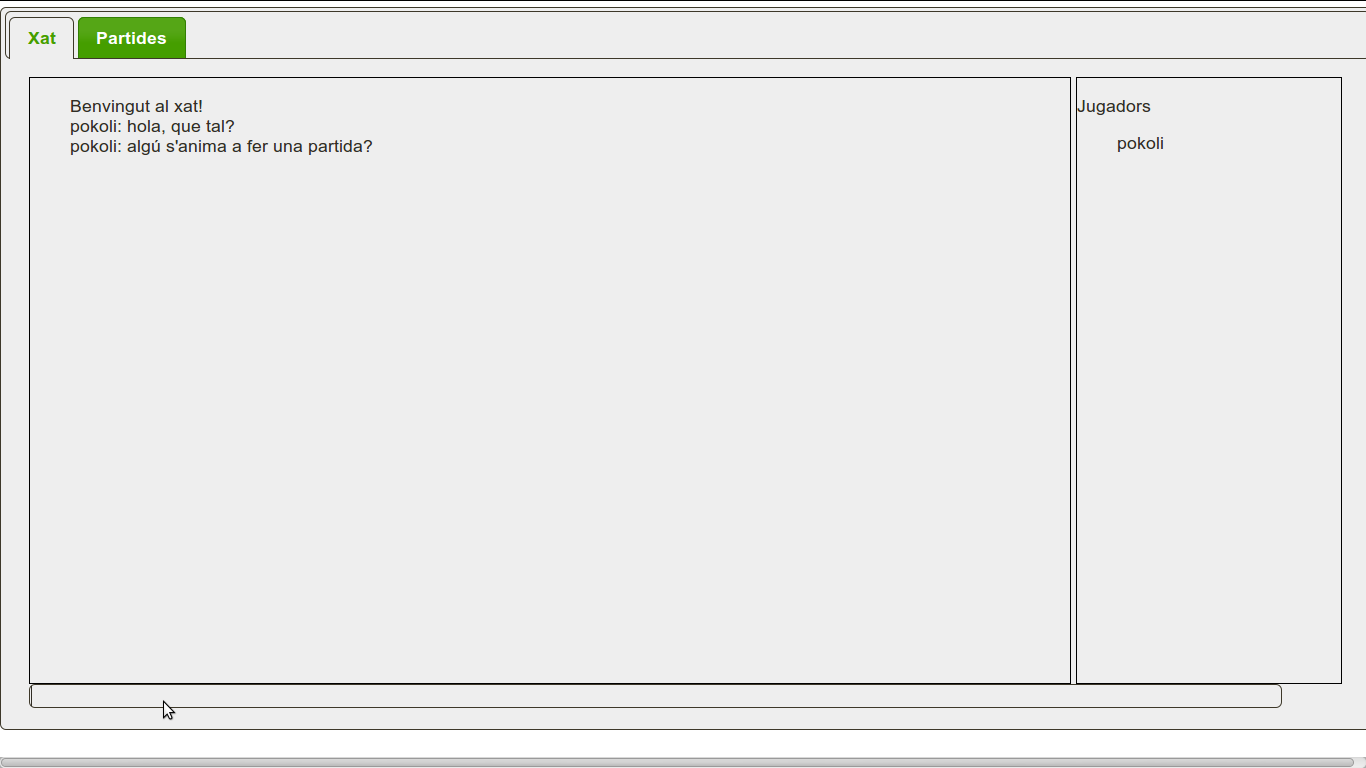
\includegraphics{img/real-xat.png}
\caption{Captura de la pantalla de xat i llista d'usuari.}
\label{fig:real-xat}
\end{figure} 

A la figura \ref{fig:real-partida} es pot veure l'aspecte que té l'aplicació en mig d'una partida. Així podem veure les nostres cartes, que clicarem per jugar quan sigui el nostre torn, juntament amb les cartes que han jugat els nostres rivals. A la part de la dreta també podem observar les dades generals de la partida, i la puntuació de les rondes que s'han jugat fins al moment. 
\begin{figure}[htbp]
\centering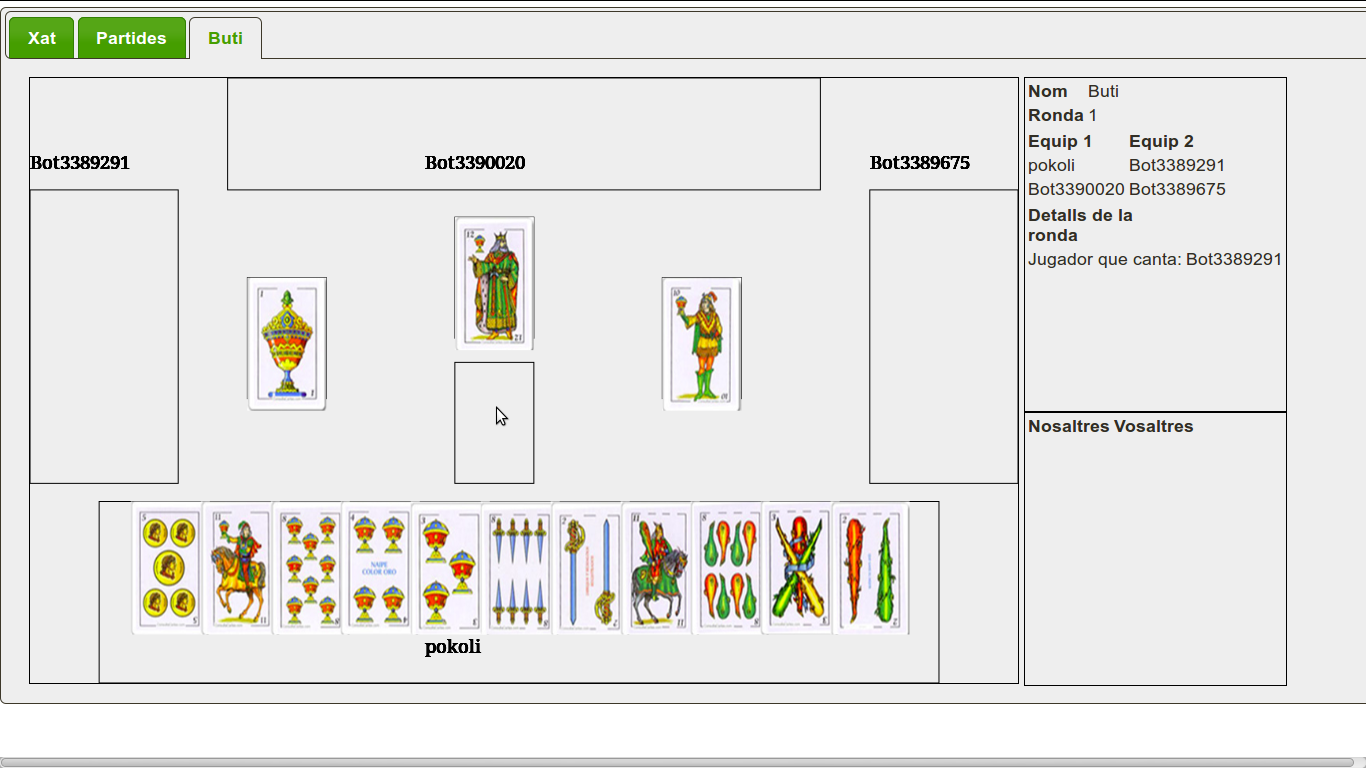
\includegraphics{img/real-partida.png}
\caption{Maqueta de la pantalla de detall de la partida}
\label{fig:real-partida}
\end{figure} 


\section{Visualització de la informació}
\label{sec:visualitzacio-informacio}

Com ja s'ha comentat anteriorment, el programa encarregat de mostrar la informació a l'usuari s'ha implementat de forma separada per tal de poder permetre múltiples tipus de client. El client per defecte s'ha escrit utilitzant una interfície web. Així, aquest programa s'encarrega de mostrar en una pàgina web la formació que es rebi a través del programa client.

Per tal de poder dibuixar l'àrea de joc de la partida i les cartes que juguen cada jugador s'ha utilitzat l'objecte canvas introduït en la última versió del llenguatge HTML. Aquest objecte proporciona un espai on poder realitzar dibuixos de forma dinàmica a través de JavaScript. Gràcies a que s'escriu a través de JavaScript ens permet dibuixar-hi sense tenir que tornar a carregar la pàgina. Aquest fet provoca que l'usuari pugui veure moviment a la pantalla. 

En la implementació per defecte, l'objecte canvas forma tot un conjunt independentment del nombre d'objectes que tenim dibuixat al seu interior. Així només és pot associar esdeveniments a l'objecte en canvas i no als elements que estan continguts al seu interior. Un dels requisits del joc es que es puguin associar esdeveniments a objectes de dins del canvas, per exemple associar un esdeveniments que cada vegada que es faci clic sobre una carta s'enviï una petició al servidor sol·licitant que es vol jugar. Per tal de solucionar aquest problema s'ha utilitzat la llibreria kinetic.js\footnote{\url{http://www.kineticjs.com/}}. A més d'associar esdeveniments als objectes de dins aquesta llibreria ens permet estructurar el dibuix a nivell de capes, permetent-nos crear tantes capes com es cregui necessari. La llibreria s'encarrega de superposar totes les capes i mostrar-les a l'usuari. 
